\documentclass[tikz, border=3pt]{standalone}

\usepackage{amsmath,amssymb}
\usepackage{pgfplots}
\pgfplotsset{compat=1.18}
\usepgfplotslibrary{groupplots}
\usetikzlibrary{arrows.meta}
\usepackage{xcolor}

\definecolor{utnblue}{RGB}{0, 51, 102}
\definecolor{utnred}{RGB}{204, 0, 0}

% Eje horizontal en unidades de pi rad/muestra
\pgfplotsset{
    espectro/.style={
        axis lines=middle,
        width=13cm, height=4.6cm,
        xmin=-3.4, xmax=3.4,
        ymin=-500, ymax=6200,
        ytick={2500,5000},
        yticklabels={$2500$,$5000$},
        xtick={-2,-1,0,1,2},
        xticklabels={$-2\pi$,$-\pi$,,$\pi$,$2\pi$},
        tick label style={font=\tiny},
        label style={font=\scriptsize},
        title style={font=\scriptsize, at={(axis description cs:1,1)},
                     anchor=north east, xshift=-2pt, yshift=-2pt},
        xticklabel style={fill=white, inner sep=1.5pt},
        every axis x label/.style={at={(ticklabel* cs:1)}, anchor=west},
        every axis y label/.style={at={(ticklabel* cs:1)}, anchor=south},
        enlargelimits=false,
        clip mode=individual,
        axis on top,
        xlabel={$\lambda$},
        ylabel={$X_s$},
    },
}

\begin{document}
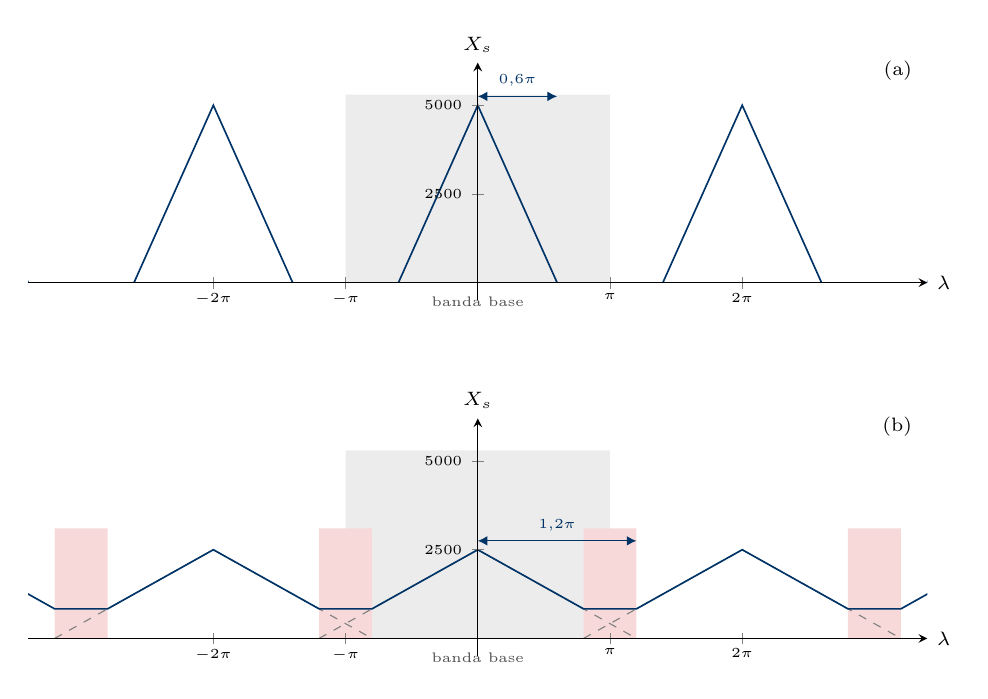
\begin{tikzpicture}[font=\scriptsize, >={Latex[length=3.5pt,width=3.5pt]}]

\begin{groupplot}[
    group style={group size=1 by 2, vertical sep=1.5cm},
    espectro,
]

% =========== (a) Delta t = 0,2 ms : la copia llega a 0,6 pi ===========
\nextgroupplot[title={(a)}]

% banda base
\addplot[draw=none, fill=gray!15] coordinates {(-1,0) (1,0) (1,5300) (-1,5300)} \closedcycle;

% copias
\addplot[utnblue, semithick] coordinates {(-4.6,0) (-4,5000) (-3.4,0)};
\addplot[utnblue, semithick] coordinates {(-2.6,0) (-2,5000) (-1.4,0)};
\addplot[utnblue, semithick] coordinates {(-0.6,0) (0,5000)  (0.6,0)};
\addplot[utnblue, semithick] coordinates {(1.4,0)  (2,5000)  (2.6,0)};
\addplot[utnblue, semithick] coordinates {(3.4,0)  (4,5000)  (4.6,0)};

% cuanto ocupa una copia
\draw[utnblue, <->] (axis cs:0,5250) -- (axis cs:0.6,5250);
\node[utnblue, font=\tiny, anchor=south] at (axis cs:0.3,5250) {$0{,}6\pi$};

\node[gray!60!black, font=\tiny, anchor=north] at (axis cs:0,-120) {banda base};

% =========== (b) Delta t = 0,4 ms : la copia llega a 1,2 pi ===========
\nextgroupplot[title={(b)}]

% banda base
\addplot[draw=none, fill=gray!15] coordinates {(-1,0) (1,0) (1,5300) (-1,5300)} \closedcycle;

% zonas de solapamiento
\addplot[draw=none, fill=utnred!15] coordinates {(0.8,0) (1.2,0) (1.2,3100) (0.8,3100)} \closedcycle;
\addplot[draw=none, fill=utnred!15] coordinates {(-1.2,0) (-0.8,0) (-0.8,3100) (-1.2,3100)} \closedcycle;
\addplot[draw=none, fill=utnred!15] coordinates {(2.8,0) (3.2,0) (3.2,3100) (2.8,3100)} \closedcycle;
\addplot[draw=none, fill=utnred!15] coordinates {(-3.2,0) (-2.8,0) (-2.8,3100) (-3.2,3100)} \closedcycle;

% copias individuales
\addplot[gray, dashed, thin] coordinates {(-3.2,0) (-2,2500) (-0.8,0)};
\addplot[gray, dashed, thin] coordinates {(-1.2,0) (0,2500)  (1.2,0)};
\addplot[gray, dashed, thin] coordinates {(0.8,0)  (2,2500)  (3.2,0)};

% suma de todas las copias
\addplot[utnblue, semithick] coordinates {
    (-4,2500) (-3.2,833) (-2.8,833) (-2,2500) (-1.2,833) (-0.8,833)
    (0,2500) (0.8,833) (1.2,833) (2,2500) (2.8,833) (3.2,833) (4,2500)
};

% cuanto ocupa una copia
\draw[utnblue, <->] (axis cs:0,2750) -- (axis cs:1.2,2750);
\node[utnblue, font=\tiny, anchor=south] at (axis cs:0.6,2750) {$1{,}2\pi$};

\node[gray!60!black, font=\tiny, anchor=north] at (axis cs:0,-120) {banda base};

\end{groupplot}

\end{tikzpicture}
\end{document}
